%\documentclass[12pt,a4paper]{report}
\documentclass[12pt,a4paper,oneside,onecolumn,openright]{book}
% set the document language
\usepackage[italian]{babel}
% set the encoding used by your editor here (default is utf8)
\usepackage[utf8]{inputenc}
\usepackage[T1]{fontenc}

% math packages
\usepackage{amsmath}
\usepackage{amssymb}
% page margins settings
\usepackage[inner=3cm,outer=2.5cm,top=3cm,bottom=2.5cm]{geometry}
%\usepackage{indentfirst}

% other packages
\usepackage{array}
\usepackage{subfigure}
\usepackage{graphicx}
\usepackage{verbatim}
\usepackage{listings}
\usepackage{url}
\usepackage[hidelinks]{hyperref}
% custom colors
\usepackage{color}
\definecolor{light-gray}{gray}{0.96}
\definecolor{cyan}{RGB}{230,230,255}
\definecolor{dkgreen}{rgb}{0,0.6,0}
\definecolor{gray}{rgb}{0.5,0.5,0.5}
\definecolor{mauve}{rgb}{0.58,0,0.82}

% environment for bash code
\lstset{ %
  language=bash,                % the language of the code
  basicstyle=\footnotesize,           % the size of the fonts that are used for the code
  numbers=left,                   % where to put the line-numbers
  numberstyle=\footnotesize,          % the size of the fonts that are used for the line-numbers
  stepnumber=1,                   % the step between two line-numbers. If it's 1, each line 
                                  % will be numbered
  numbersep=5pt,                  % how far the line-numbers are from the code
  backgroundcolor=\color{white},      % choose the background color. You must add \usepackage{color}
  showspaces=false,               % show spaces adding particular underscores
  showstringspaces=false,         % underline spaces within strings
  showtabs=false,                 % show tabs within strings adding particular underscores
%  frame=single,                   % adds a frame around the code
  rulecolor=\color{black},        % if not set, the frame-color may be changed on line-breaks within not-black text (e.g. commens (green here))
  tabsize=2,                      % sets default tabsize to 2 spaces
  captionpos=b,                   % sets the caption-position to bottom
  breaklines=true,                % sets automatic line breaking
  breakatwhitespace=false,        % sets if automatic breaks should only happen at whitespace
  title=\lstname,                   % show the filename of files included with \lstinputlisting;
                                  % also try caption instead of title
  numberstyle=\tiny\color{gray},        % line number style
  keywordstyle=\textbf,          % keyword style
  commentstyle=\color{dkgreen},       % comment style
%  stringstyle=\color{mauve},         % string literal style
  escapeinside={\%*}{*)},            % if you want to add a comment within your code
  morekeywords={*,...,insert,-}               % if you want to add more keywords to the setù
}

% environment for python code
\lstset{
language=Python,
breaklines=true,
breakatwhitespace=true ,
backgroundcolor=\color{light-gray}
}
% appendices package
%\usepackage{appendix}
% set Appendix name used in the toc
%\renewcommand{\appendixtocname}{Appendice}

% interline
\linespread{1.5}
% set numbers for subsections and show them in the toc
\setcounter{tocdepth}{3} 
\setcounter{secnumdepth}{3}

% layout package, style and settings
\usepackage{fancyhdr}
\pagestyle{fancy}

\fancypagestyle{mainmatter}{%		
		\fancyhf{} 
		\fancyhead{}
		\fancyhead[LE,RO]{\thepage}
		\fancyhead[LO]{\footnotesize{\leftmark}}
		\fancyhead[RE]{\footnotesize{\rightmark}}
		\fancyfoot{}
		\addtolength{\headwidth}{\marginparsep}
		\addtolength{\headheight}{2.5pt}
		\renewcommand{\headrulewidth}{0.3pt}
		\renewcommand{\footrulewidth}{0.0pt}
		}
\fancypagestyle{frontmatter}{%
		\fancyhf{} 
		\fancyhead[LE]{\footnotesize{\MakeUppercase{\thepage}}}
		\fancyhead[RO]{\footnotesize{\MakeUppercase{\thepage}}}
		\fancyhead[RE,LO]{}
		\fancyfoot{}
		\addtolength{\headwidth}{\marginparsep}
		\addtolength{\headheight}{2.5pt}
		\renewcommand{\headrulewidth}{0.0pt}
		\renewcommand{\footrulewidth}{0.0pt}
		}
		
		
\usepackage{fancyhdr}
\pagestyle{fancy}
		\fancyhf{} 
		\fancyhead{}
		\fancyhead[LE,RO]{\thepage} 
		\fancyhead[LO]{\footnotesize{\leftmark}}
		\fancyhead[RE]{\footnotesize{\rightmark}}
		\fancyfoot{}
		\addtolength{\headwidth}{\marginparsep}
		\addtolength{\headheight}{2.5pt}
		\renewcommand{\headrulewidth}{0.3pt}
		\renewcommand{\footrulewidth}{0.0pt}

% empty pages have no numbers
\makeatletter
\def\cleardoublepage{\clearpage\if@twoside \ifodd\c@page\else
\hbox{}
  %Potresti voler togliere il commento dalla linea seguente
  %Questa pagina � stata lasciata intenzionalmente vuota.
\thispagestyle{empty}
\newpage
\if@twocolumn\hbox{}\newpage\fi\fi\fi}
\makeatother
%????
%\textwidth=450pt\oddsidemargin=0pt

%\makeatletter 
%  \DeclareRobustCommand*\textsubscript[1]{% 
%    \@textsubscript{\selectfont#1}} 
%  \newcommand{\@textsubscript}[1]{% 
%    {\m@th\ensuremath{_{\mbox{\fontsize\sf@size\z@#1}}}}} 
\makeatother 

\begin{document}
\begin{titlepage}
\begin{center}
{
    \large
    \textbf{Università  degli studi di Modena e Reggio Emilia} \\
   	\textbf{Dipartimento di Ingegneria "Enzo Ferrari"} \\
    \vspace{\stretch{0.5}}
    \hspace*{0cm} \hrulefill \hspace*{0cm} \\
    \vspace{\stretch{0.5}}
   	\emph{Corso di Laurea in Ingegneria Informatica - Sede di Mantova}
    
	  \vspace{\stretch{12}}
  
  
 		\huge{\bf Titolo: prima riga }}\\
		\vspace{3mm}
		{\huge{\bf Seconda riga}}\\
		\vspace{3mm}
		\vspace{3mm}
		{\huge{\bf Terza riga}}\\
		\vspace{3mm}
		\vspace{3mm}
		{\huge{\bf Quarta riga}}\\
		
		\vspace{\stretch{6}}
		\end{center}
		
\vspace{40mm}
\par
\noindent
\begin{minipage}[t]{0.47\textwidth}
{\large{\bf Relatore:\\
Prof. Luca Ferretti}}\\ 
\\
{\large{\bf Correlatore:\\
Ing. Federico Magnanini}}
\end{minipage}
\hfill
\begin{minipage}[t]{0.47\textwidth}\raggedleft
{\large{\bf Candidato:\\
Giulio Barabino}}
\end{minipage}
\vspace{20mm}
\begin{center}
%\rule[0.1cm]{15.8cm}{0.1mm}
\hspace*{0cm} \hrulefill \hspace*{0cm} \\
{\large{\bf 
Anno Accademico 2021/2022}}
\end{center}

\end{titlepage}

\pagestyle{frontmatter}
\frontmatter

% PAGINA VUOTA
%\clearpage\null\thispagestyle{empty}\clearpage
\setcounter{tocdepth}{2}
\tableofcontents

\setlength{\parindent}{12pt}
\setlength{\parskip}{1ex plus 0.5ex minus 0.2ex}
\mainmatter
\pagestyle{mainmatter}

\chapter{Introduzione}
\label{intro}

Il Single Sign-On è un protocollo utilizzato per migliorare e semplificare il processo di autenticazione. Alleggerisce i servizi Web che lo utilizzano dall'onere di gestire la moltitudine di credenziali degli utenti, con i meccanismi di protezione necessari che ne conseguono. I protocolli di SSO possono autenticare gli utenti mediante protocolli passwordless. Grazie a questi protocolli un utente effettua l'autenticazione tramite un token hardware in grado di eseguire operazioni di autenticazione basate su crittografia asimmetrica. Questo permette di snellire e irrobustire il processo complessivo di autenticazione. Il limite principale risiede nella centralizzazione del protocollo SSO che non è in grado di tollerare intrusioni nell'infrastruttura che lo esegue.
Infatti, come mostrano attacchi recenti \cite{volexity:solarwinds} \cite{nsa:authentication}, gli attaccanti che riescono a compromettere l'infrastruttura di SSO sono in grado di impersonare utenti arbitrari.
Per mitigare questa problematica sono nati gli studi sulla cosiddetta SSO \emph{survivability}. Tale filone si occupa di irrobustire il protocollo SSO utilizzando un approccio distribuito e replicato. Si prevede un numero di attori malevoli di cui è possibile tollerare l'intromissione, numero da cui dipende il livello di sicurezza.

L'esigenza di questa tesi nasce dal fatto che i protocolli esistenti in ambito SSO \emph{survivable} non permettono di modificare il livello di sicurezza una volta che è stato stabilito durante la fase di creazione dell'infrastruttura. Questo impedisce ai vari servizi Web di richiedere alla stessa infrastruttura SSO livelli di sicurezza adeguati alle caratteristiche del servizio offerto. Si è affrontato dunque il problema dell'integrazione del livello di sicurezza all'interno dei protocolli Passwordless e SSO preesistenti. A tal fine, si è reso necessario implementare modifiche al codice di un autenticatore open source, cui hanno fatto seguito verifiche delle performance di autenticazione e un breve studio di fattibilità per l'implementazione su hardware reale.

La tesi è strutturata nel seguente modo: nel capitolo \ref{conoscenze} vengono introdotte le conoscenze necessarie per proseguire nella lettura dei successivi; il capitolo \ref{modellazione} di modellazione in cui vengono descritti gli attori che partecipano al protocollo di SSO proposto, il funzionamento dei protocolli citati e la soluzione studiata per integrare il livello di sicurezza; il capitolo \ref{dettagli} in cui vengono approfondite le modifiche apportate al codice degli attori presenti per realizzare l'integrazione; il capitolo \ref{prestazioni} di analisi dei dati raccolti, valutazione delle tempistiche e studio finale di fattibilità; il capitolo \ref{conclusioni} conclusivo con le considerazioni finali ed eventuali sviluppi futuri.

\chapter{Conoscenze di Base}
\label{conoscenze}

In questa sezione verranno introdotti i concetti necessari per proseguire con la lettura dei capitoli successivi. 

\section{Crittografia asimmetrica}
\label{asimmetrica}

La crittografia asimmetrica è un tipo di crittografia in cui ogni attore possiede una coppia di chiavi: una \textbf{pubblica} e una \textbf{privata}. Gli usi della crittografia asimmetrica sono due:
\begin{itemize}
	\item Cifrare le comunicazioni: tramite la chiave pubblica del destinatario è possibile cifrare un messaggio che solo il destinatario può decifrare usando la propria chiave privata.
	\item Firmare digitalmente: tramite la propria chiave privata un attore può apporre su un messaggio, autenticandolo, la firma, la quale può essere verificata tramite la chiave pubblica del firmatario.
\end{itemize}

\section{Single Sign-On}
\label{sso}

% AGGIUNGERE ATTORI

Il \emph{Single Sign-On} è un protocollo molto diffuso utilizzato per autenticare utenti a servizi Web. Il protocollo è eseguito da un utente, un User Agent, un Identity Provider e un Service Provider. L'User Agent è un software usato dall'utente che permette l'interazione con un contenuto Web. L'Identity Provider è un attore terzo che si occupa di fornire un sistema di autenticazione sicuro, creando e gestendo le credenziali degli utenti, a servizi Web che lo richiedano. L'Identity Provider possiede degli Identity Server presso cui gli utenti devono eseguire le operazioni di autenticazione. Il Service Provider è un fornitore di servizio Web che non implementa sistemi di autenticazione propri ma utilizza quelli messi a disposizione dall'Identity Provider. Qualora l'utente si autentichi con successo presso l'Identity Server gli viene fornito un token di autenticazione firmato dell'Identity Server, che deve presentare al Service Provider per poter fruire di quel servizio.  Una volta presentato il token al Service Provider sarà autenticato a tutti quei servizi messi a disposizione dal Service Provider che fanno uso dello stesso Identity Provider, da qui l'accezione \emph{single} di \emph{sign-on}.

\section{Survivability}
\label{surviv}

La centralizzazione dello schema SSO lascia spazio ad attacchi in cui un malintenzionato prenda il controllo dell'Identity Server e utilizzi la chiave privata dello stesso per firmare token di autenticazione forgiati arbitrariamente, così da poter poi impersonare qualunque utente egli voglia. Vengono in aiuto gli schemi cosiddetti \emph{survivable SSO} che possono limitare tali criticità sfruttando più Identity Server. Un singolo Identity Provider gestisce quindi più Identity Server e l'utente deve autenticarsi presso un sottoinsieme di questi, i quali rilasciano poi un \textbf{token} firmato collettivamente. 

La componente survivable risiede nel fatto che viene tollerato un certo numero di Identity Server violati e, di conseguenza, viene richiesto un token in funzione di questo numero. Con una soglia di tolleranza di server maligni sufficiente si riesce a garantire l'integrità del meccanismo di autenticazione e un overhead, dovuto alla reiterazione dei passaggi, trascurabile.

\section{Passwordless}
\label{passwordless}

L'autenticazione passwordless è un metodo di autenticazione che permette ad un utente di effettuare il login ad un servizio senza la necessità di conoscere una password o più genericamente una conoscenza considerata segreta. Tipicamente utilizza una coppia di chiavi crittografiche, una privata e una pubblica: la prima è generata e immagazzinata sul dispositivo dell'utente, mentre la seconda è inviata al server così che esso possa verificare l'autenticità dei messaggi ricevuti. La chiave privata, o segreta, non lascia mai il dispositivo su cui è stata creata e per accedervi è necessaria l'autorizzazione ottenuta tramite \textbf{mediazione} da parte dell'utente. Un'azione è detta mediata da un utente qualora sia necessario il suo esplicito consenso. Il consenso può avvenire, ad esempio, premendo il bottone sul dispositivo fisico.

La registrazione passwordless e, conseguentemente, l'autenticazione vengono svolte seguendo un meccanismo \emph{challenge-response}: al pervenire di una richiesta di registrazione il server invia una cosidetta \emph{challenge}. L'utente che ha iniziato l'operazione ha il compito di apporre, tramite propria chiave privata, una firma crittografica sulla challenge e di fornire in risposta al server la challenge firmata accompagnata dalla chiave pubblica. Così facendo il server verifica l'autenticità della firma tramite la chiave appena ricevuta e in caso di esito positivo immagazzina la chiave pubblica. La fase di autenticazione è svolta in modo analogo con la differenza che il server è già in possesso della chiave pubblica e non è quindi necessario inviarla.

Come si può vedere non viene scambiato alcun segreto e l'unica interazione richiesta all'utente è quella in fase di firma della challenge. Anche allora l'utilizzatore non deve inserire codici o password ma semplicemente mediare l'operazione tramite uno dei metodi sopra elencati. Sfruttando l'autenticazione passwordless è possibile sopperire alle criticità tipiche dei segreti a bassa entropia come le password, quali phishing, brute forcing etc. 

\section{FIDO}
\label{fido}

FIDO Alliance è un'associazione nata nel 2013 con lo scopo di migliorare i sistemi di autenticazione tramite la diffusione dell'autenticazione passwordless. Sono gli autori di \emph{FIDO}, un set di specifiche che include gli standard \textbf{CTAP} e \textbf{WebAuthn}. Nel corso degli anni vi sono stati un susseguirsi di iterazioni degli standard, prima conosciuta come Universal Authentication Factor per poi diventare Universal 2nd Factor e giungere infine alla versione corrente FIDO 2.0. 

Il protocollo CTAP definisce le API che un client può utilizzare per comunicare con un autenticatore. Il protocollo WebAuthn si occupa invece di definire le API per l'autenticazione a servizi web sfruttando le chiavi crittografiche. 

In particolare definiscono tutto il necessario per programmare un autenticatore e un server come: strutture dati, metodi, requisiti di funzionamento, encoding dei dati etc.

\subsection{Rilevamento tentativi di clonazione}
\label{fido:clonazione}

Compito dell'Identity Server è anche quello di rilevare eventuali tentativi di duplicazione dell'autenticatore fisico. Per fare ciò lo standard FIDO prevede un \textbf{contatore}, sia esso globale o multiplo, aggiornato dall'autenticatore ad ogni operazione avvenuta con successo. Il contatore prende il nome di \emph{signature counter}. Il server mantiene in memoria l'ultimo valore ricevuto e, all'interazione successiva, controlla che non vi siano discrepanze. Ad esempio, ipotizzando di avere allo stesso tempo:
\begin{itemize}
	\item Un autenticatore originale con contatore pari a \emph{m}
	\item Un autenticatore clone dell'originale con contatore pari a \emph{m}
\end{itemize}
Se l'autenticatore originale si autentica presso un servizio, questi aggiorna il proprio contatore a ${m+1}$. Il clone, tentando di autenticarsi allo stesso servizio, fornisce un valore del contatore pari a \emph{m}, dunque minore di quello salvato in memoria dal server al momento dell'ultima interazione con l'autenticatore originale. In questo modo, il server riconosce il clone in quanto tale. 

Ne consegue che il rilevamento del tentativo di clonazioni basato sul contatore risulta:
\begin{itemize}
	\item Inefficace finché il clone non procede ad autenticarsi
	\item Fallace se il clone procede ad autenticarsi prima dell'originale: quest'ultimo viene di fatto invalidato nonostante sia legittimo
\end{itemize} 
\chapter{Modellazione del sistema}
\label{modellazione}

In questo capitolo verranno inizialmente descritti gli attori che concorrono alle fasi di registrazione/autenticazione per poi definire il flusso delle operazioni stesse.

\section{Attori}
\label{attori}

Lo schema di seguito rappresenta lo stato attuale dello standard FIDO in accordo all'implementazione descritta successivamente.
\begin{figure}[htb]
	\centering
	
\includegraphics[width=.4\columnwidth]{figures/example.pdf}
	\caption{PLACEHOLDER.}
	\label{fig:esempio}
\end{figure}
% INSERIRE SCHEMA ATTORI STATO ATTUALE

\subsection{Service Provider}
\label{service_provider}

Il Service Provider è un fornitore di un generico servizio a cui l'utente è interessato ad accedere. Può essere un qualunque servizio di streaming, banking, shopping etc. il quale fa uso di un intermediario per l'autenticazione dei propri utenti. Questo può avvenire per varie ragioni sia economiche che legate alla sicurezza. 

Il Service Provider fa uso del \textbf{security level} per indicare il livello di \emph{survivability} desiderato: esso può crescere all'aumentare della confidenzialità del servizio erogato.

\subsection{Identity Provider}
\label{identity_provider}

L'Identity Provider è un ente terzo che si occupa di fornire a un Service Provider il servizio di autenticazione. Fa parte del cosiddetto \emph{Relying Party}, cioè quella parte che fornisce un accesso sicuro ad un servizio. 

Nella variante \emph{survivable}, invece che fornire un Identity Server unico con il quale il FIDO Client comunica, ne fornisce un numero \textbf{n} desiderato dal Service Provider, a seconda della sicurezza richiesta dal tal servizio. In questo modo durante la fase di creazione l'operazione dovrà essere replicata dal client su tutti gli \emph{n} Identity Server. La parte di autenticazione invece verrà svolta solo su un sottoinsieme $\mathbf{k\leq n}$ di questi. Compito dell'Identity Provider è anche quello di fornire il token di autenticazione al client da presentare al Service Provider per fare in modo che l'utente possa accedere al servizio scelto.

I vari Identity Server comunicano con il FIDO Client, tramite User Agent, per creare le credenziali degli utenti mantenendo in memoria le challenge generate e gli identificatori degli utenti registrati con le relative chiavi pubbliche ricevute. 

Compito dell'Identity Server è anche quello di rilevare eventuali tentativi di duplicazione dell'autenticatore fisico. Per fare ciò lo standard FIDO prevede un contatore gestito dall'autenticatore, sia esso globale o multiplo, che viene aggiornato ad ogni operazione avvenuta con successo. Il contatore prende il nome di \emph{signature counter}. Il server mantiene in memoria l'ultimo valore ricevuto e, all'interazione successiva, controlla che non vi siano discrepanze. In particolare se il valore ricevuto è minore di quello salvato in memoria dal server allora si può essere in presenza di un tentativo di clonazione. (L'accadere dell'inverso non è detto che costituisca un problema, motivo per il quale può essere utilizzato anche un contatore globale.) Ciò significa che un attaccante maligno ha duplicato l'autenticatore ad uno stato precedente mentre l'utilizzatore ha continuato ad autenticarsi incrementando il contatore. 

Nella variante survivable è stato modellato il sistema adottando un contatore specifico per ogni livello di sicurezza. Ad ogni autenticazione, e quindi ad ogni livello di sicurezza desiderato specificato dal Service Provider, verrà incrementato il contatore corrispondente a \emph{k}. Questa modifica non altera il funzionamento del server, che riceve sempre un valore di contatore unico, indi per cui non è stato necessario operare modifiche in questo senso dal lato del server.

\subsection{Autenticatore}
\label{autenticatore}

L'autenticatore hardware è un dispositivo che, tramite l'interazione fisica con l'utente, permette l'accesso al servizio web richiesto. Durante la fase di creazione delle credenziali, l'autenticatore si occupa di creare una coppia di chiavi crittografiche, una pubblica e una privata. Utilizzerà la chiave privata per firmare le challenge che gli vengono sottoposte mentre la pubblica verrà inviata al server così che esso possa verificare l'autenticità delle firme.

Per la fase di creazione e le successive di autenticazione viene richiesto all'utente di compiere un'azione: essa può essere la pressione di un pulsante sulla chiavetta stessa, un collegamento NFC oppure ancora l'identificazione tramite impronta digitale. Così facendo l'operazione in corso viene autenticata.

Nella variante \emph{survivable} viene inviato il digest ottenuta dall'hashing delle \emph{n} challenge dei server che partecipano all'operazione. Esso appare all'autenticatore come una challenge unica, motivo per il quale non è stato necessario modificare il codice dell'autenticatore per richiedere l'interazione ad ogni singola challenge. 

Durante la fase di registrazione viene inizializzato un contatore tramite cui vengono tenute traccia delle operazioni conseguite correttamente. Ad ogni operazione il contatore, al corrispondente livello di sicurezza, viene incrementato mono-atomicamente. Come detto in precedenza, si è reso necessario implementare un contatore specifico per ogni livello di sicurezza richiesto, sia in fase di autenticazione che di creazione. Prima di fare ciò, è stato però necessario introdurre un contatore per ogni credenziale creata, poiché allo stato attuale il codice della Solokey, per questioni di spazio, prevede un contatore globale unico. 

\subsection{Client}
\label{client}

Un dispositivo client che sfrutta un User Agent conforme ad implmentare le specifiche FIDO per il dialogo con il Relying Party e con l'autenticatore, in collaborazione con il dispositivo hardware sottostante su è installato l'User Agent, tipicamente un sistema operativo. Il client è quindi interposto tra il FIDO Server e l'autenticatore fisico, agendo da intermediario. Il suo compito è duplice:
\begin{itemize}
	\item Comunicare con il server al fine di iniziare, e successivamente terminare, le operazioni di autenticazione e di creazione delle credenziali 
	\item Comunicare con l'autenticatore allo scopo di creare le chiavi crittografiche e firmare le challenge ricevute dal server
\end{itemize}
La comunicazione è bidirezionale, duplice e segue i costrutti specificati dalle API definite nei relativi standard: CTAP per l'interazione con l'autenticatore e WebAuthn per la comunicazione con il FIDO Server. 

Nel caso particolare dell'estensione survivable il client si occupa di replicare le operazioni su \emph{n} FIDO Server distinti, computando l'hash delle challenge ricevute e fornendolo all'autenticatore come un digest unico su cui apportare la firma. 

\section{Flusso operativo}
\label{flusso_operativo}

Il flusso operativo si compone di due operazioni distinte: una fase di creazione delle credenziali e una fase di autenticazione dell'utente. Tali operazioni vengono svolte, rispettivamente, durante la registrazione al servizio del Service Provider e a tutti i login successivi.

\subsection{Fase di registrazione}
\label{registrazione}

La fase di registrazione si origina a partire dalla richiesta dell'utente, utilizzando un User Agent, di registrarsi ad un servizio, offerto da un Service Provider, che supporti l'autenticazione passworldess, tramite degli Identity Provider. Il Service Provider fornisce all'utente il livello di sicurezza \emph{n} necessario per completare l'operazione. Il processo messo in atto è il seguente:

\begin{enumerate}
	\item Ogni Identity Server crea il proprio stato interno e la challenge
	\item Ogni Identity Server invia al Client una serie di requisiti secondo cui deve essere svolta la cerimonia di registrazione, e la challenge generata
	\item Il Client salva tutte le challenge ricevute in un vettore e computa l'hash dello stesso
	\item Il Client effettua una chiamata al metodo opportuno dell'autenticatore, fornendo i requisiti di creazione richiesti dal Relying Party e il digest computato come challenge
	\item L'autenticatore procede a generare la coppia di chiavi crittografiche seguendo le imposizioni del server e invia al client la challenge firmata accompagnata dalla chiave pubblica e dal signature counter
	\item Il Client invia ad ogni Identity Server il vettore con le challenge, l'hash dello stesso, la firma. la chiave pubblica e il signature counter ricevuto
	\item Ogni Identity Server controlla che la challenge da lui generata sia presente all'interno del vettore e controlla, computando lui stesso l'hash del vettore, l'integrità di quanto ricevuto. Infine, verifica tramite la chiave pubblica fornitagli l'autenticità della firma.
	\item Qualora il processo sia andato a buon fine, gli Identity Server salveranno le informazioni ricevute (contatore, chiave pubblica, identificatore del client) al proprio interno e forniranno al Client l'attestazione con cui poter completare la registrazione presso il Service Provider
\end{enumerate} 

\subsection{Fase di autenticazione}
\label{autenticazione}

La fase di autenticazione ricalca i passaggi di quella di registrazione con la differenza che gli Identity Server sono già in possesso della chiave pubblica con cui verificare l'autenticità della firma apportata alle challenge. 

In questa fase viene comunicato un security level pari a \emph{k} da parte del Service Provider, cioè il numero di Identity Server presso cui è necessario autenticarsi. Questo valore prende in considerazione la tollerabilità alle intrusione che ha il Service Provider. In particolare: \emph{k} può essere $ \emph{(2j+1)} $, dove \emph{j} rappresenta il numero di Identity Server di cui si può tollerare la compromissione, oppure può essere $ \emph{(2j+2)} $ in caso di requisiti particolarmente stringenti. 

\begin{enumerate}
	\item Ogni Identity Server crea il proprio stato interno e la challenge
	\item Ogni Identity Server invia al Client una serie di requisiti, secondo cui deve essere svolta la cerimonia di autenticazione, e la challenge generata
	\item Il Client salva tutte le challenge ricevute in un vettore e computa l'hash dello stesso
	\item Il Client effettua una chiamata al metodo opportuno dell'autenticatore, fornendo i requisiti di autenticazione richiesti dal Relying Party e il digest computato come challenge
	\item L'autenticatore invia al Client la challenge firmata e il contatore, specifico del livello di sicurezza stabilito, aggiornato
	\item Il Client invia ad ogni Identity Server il vettore con le challenge, l'hash dello stesso, la firma ricevuta e il signature counter
	\item Ogni Identity Server controlla che la challenge da lui generata sia presente all'interno del vettore e controlla, computando lui stesso l'hash del vettore, l'integrità di quanto ricevuto. Infine, verifica tramite la chiave pubblica, memorizzata precedentemente, l'autenticità della firma
	\item Ogni Identiy Server controlla che il \emph{signature counter} ricevuto sia maggiore di quello memorizzato in precedenza e in tal caso aggiorna quest'ultimo
	\item Se i passaggi precedenti sono avvenuti con successo rilasciano al Client l'attestazione tramite cui può completare l'autenticazione presso il Service Provider
\end{enumerate}
\chapter{Dettagli}
\label{dettagli}

In questo capitolo si trattano i dettagli implementativi relativi alle modifiche operate a:
\begin{itemize}
	\item Una variante della libreria FIDO2 realizzata da Yubico modificata in una tesi precedente per accogliere il meccanismo survivable \cite{yubico:fido}
	\item Il codice sorgente dell'autenticatore Solokeys \cite{solokeys:code} per integrare il \emph{security level}
\end{itemize}

Nonostante la libreria Yubico fosse già stata modificata in precedenza per adottare la struttura survivable, è stato comunque necessario operare cambiamenti. La libreria FIDO2 si occupa di simulare l'interazione tra un Client FIDO2 e un Server FIDO2 per emulare la registrazione e la successiva autenticazione. Grazie alla modifica apportata precedentemente è possibile simulare un numero arbitrario di Server con cui stabilire la comunicazione e svolgere tali operazioni. Tutto il funzionamento descritto nel capitolo precedente è correttamente gestito, ad esclusione dell'invio del security level.

Lato autenticatore invece si è reso necessario implementare diverse funzionalità: dal parsing del security level nel messaggio inviato dall'User Agent all'autenticatore fino ad arrivare a un contatore globale vero e proprio. Infatti, da standard FIDO2 il signature counter utilizzato per il controllo della clonazione dell'autenticatore può essere anche globale e non specifico per credenziale \cite{fido:signature_counter}. Ciò è dovuto alla natura \emph{constraint}, cioè con limitazioni di memoria importanti, degli autenticatori hardware.

\section{Modifica della libreria FIDO2}
\label{modifica_fido}

La libreria FIDO2 presenta il file \verb*|client_multichallenge.py| in cui viene definita la classe \verb*|Fido2ClientMultichallenge|, figlia della classe \verb*|Fido2Client| nel relativo \verb*|client.py|, che permette l'autenticazione WebAuthn simulando un Client FIDO. Presenta due metodi, \verb*|make_credential| per realizzare l'operazione di creazione delle credenziali e \verb*|get_assertion| per compiere l'operazione di autenticazione. 

Rispetto alla condizione di partenza è stato aggiunto il controllo del contatore lato server. Per fare ciò è stato definito all'interno del costruttore di \verb*|Fido2ServerMultichallenge| un dizionario tramite cui tenere traccia dei contatori:
\begin{verbatim}
	self.counter_register = {}
\end{verbatim}
I metodi interessati della classe sono sostanzialmente due: 
\begin{itemize}
	\item \verb*|register_complete|
	\item \verb*|authenticate_complete|
\end{itemize}

Entrambe le funzioni si occupano di controllare la correttezza dei dati ricevuti dal Client dopo che ha interpellato l'autenticatore. Entrambi i metodi vengono chiamati nel file \verb*|client_multichallenge.py| e ad entrambi è stato aggiunto il passaggio del parametro \verb*|security_level|.

Nel primo metodo, \verb*|register_complete|, viene salvato il contatore ricevuto all'interno del dizionario. Per fare ciò viene creato un secondo dizionario interno al primo, utilizzando il \emph{CredentialID} ricevuto in dall'autenticatore. In questo secondo dizionario sarà presente la coppia \verb*|security_level|:\verb*|contatore|. 
\begin{verbatim}
self.counter_register[credential_id] 
    = 
      {security_level: attestation_object.auth_data.counter}
	
\end{verbatim}

Nel secondo metodo invece vengono effettuati i controlli sulla base di quanto salvato dal server nel proprio dizionario e quanto ricevuto dall'autenticatore. In caso di contatore ricevuto minore o uguale a quello immagazzinato viene sollevato un errore che porta alla terminazione del programma. 
\begin{verbatim}
	if auth_data.counter <= self.counter_register[credential_id][security_level]:
	    raise ValueError("Counter did not increase.")
\end{verbatim}
Questo perchè si suppone che vi sia stato un tentativo di clonazione. 

Qualora, invece, il contatore fosse maggiore di quello immagazzinato $+1$ allora verrà solamente notificato il fornitore del server tramite un messaggio in console di log. 
\begin{verbatim}
elif auth_data.counter > self.counter_register[credential_id][security_level] + 1:
    print("Counter bigger than expected")
\end{verbatim}
In quest'ultimo caso e nel caso in cui il contatore venga incrementato correttamente viene aggiornato il valore corrispondente nel dizionario del server. Se nessuna di queste condizioni è verificata vuol dire che non è presente nel dizionario una voce con quel dato security level: in questo caso viene semplicemente aggiunto il security level al dizionario interno con il relativo contatore.

\begin{verbatim}
	self.counter_register[credential_id][security_level] = auth_data.counter
\end{verbatim}

\begin{center}
	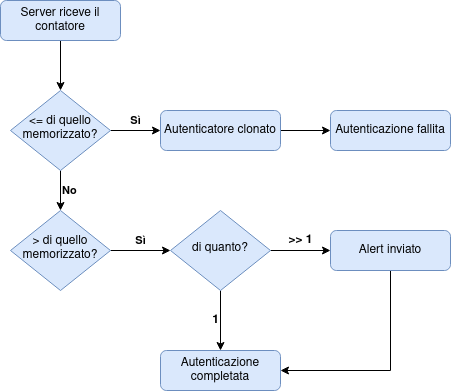
\includegraphics[width=.6\columnwidth]{figures/flowchart_contatore}
	\label{fig:contatore_webauthn}
\end{center}

\section{Modifica del codice Solo}
\label{modifica_solo}

Il codice dell'autenticatore Solokeys, come detto in precedenza, presentava un solo contatore globale per tenere traccia di tutte le operazioni di creazione/autenticazione svoltesi con successo. Il primo passo è stato, quindi, quello di implementare una struttura dati per la memorizzazione di un contatore per credenziale. Tale struttura dati, definita \verb*|signCounter| è una tipo di dato composto da due valori.
\begin{itemize}
	\item Una istanza \verb*|id| della \emph{struct} \verb*|CredentialId|
	\item Un intero senza segno di 32 bit definito come \verb*|signCount|
\end{itemize}

La struttura dati \verb*|CredentialId| definisce come vengono memorizzate le credenziali all'interno dell'autenticatore seguendo lo standard FIDO \cite{fido:credential_id}. In particolare, invece che avere una sequenza di 16 bytes come da standard, presenta valori come \begin{verbatim}
	tag, nonce, padding, metadata, rpIdHash
\end{verbatim} 

La definizione della struttura \verb*|signCounter| è effettuata all'interno del file \verb*|ctap.h| e sempre nello stesso file è inizializzato anche \verb*|signCounterArray|, cioè un array di strutture dati \verb*|signCounter|. Tramite questo array è possibile memorizzare un contatore per credenziale. 

L'array viene popolato nel momento in cui viene chiamata la funzione \verb*|ctap_make_credential| utilizzata dall'autenticatore per compiere le operazioni di creazione delle credenziali. In particolare:
\begin{itemize}
	\item tramite un intero senza segno \verb*|globalCounter| viene tenuta traccia dell'ultima posizione dell'array occupata
	\item viene istanziata una struttura dati \verb*|signCounter| con \verb*|id| pari a quello calcolato e $\verb*|signCount| = 1 $
	\item viene aggiunta la struttura dati \verb*|signCounter| all'array \verb*|signCounterArray| alla posizione \verb*|globalCounter|
\end{itemize}

Nel momento in cui viene chiamata la funzione \verb*|ctap_get_assertion| viene cercata iterativamente la struttura dati il cui \verb*|id| corrisponde a quello dell'operazione corrente e viene incrementato il contatore di tale struct. 

\begin{verbatim}
    for (uint l = 0; l <= globalCounter; l++) {
        if (count_cmp_func(&cred->credential.id, &signCounter1[l])) {
            count = update_sign_counter(&signCounter1[l], GA.securityLevel);
        }
    }
\end{verbatim}

Per verificare che l'\verb*|id| corrisponda a quello generato in fase di \verb*|get_assertion| è stato necessario scrivere una funzione di comparazione: il C, infatti, non supporta nativamente la comparazione di due struct. A tal scopo è stata scritta la funzione \verb*|count_cmp_func| che compara attributo dopo attributo tutti quelli presenti all'interno della struttura per verificarne l'uguaglianza.
Il contatore, invece, viene aggiornato tramite la funzione \verb*|update_sign_counter| che semplicemente prende il valore \verb*|signCount| passato in chiamata e restituisce $signCount + 1$.

Il passo successivo è stato quello di modificare la struttura dati \verb*|signCounter| per fare in modo che accogliesse un contatore per \emph{security level}. Per fare ciò l'attributo \verb*|signCount| è stato cambiato da intero senza segno di 32 bit ad array di interi senza segno di 32 bit. Analogamente al processo di incremento seguito prima, il contatore corrispondente al security level ricevuto verrà aggiornato nel seguente modo:
\begin{verbatim}
	update_sign_counter(signCounter.signCount[n]])
\end{verbatim}
Così facendo vengono mantenuti e incrementati \emph{n} signature counter differenti per ogni credenziale. 


L'ultimo passaggio è stato quello di ricezione del \emph{security level}. Lo standard CTAP2 \cite{fido:ctap_commands} definisce i codici dei comandi a cui deve essere associato il lancio di alcune funzioni. Ogni comando è strutturato con il proprio codice di comando e i codici per i propri parametri. I codici per per i comandi di interesse sono i seguenti: 
\begin{verbatim}
	0x01	authenticatorMakeCredential
	0x02	authenticatorGetAssertion
\end{verbatim}


L'autenticatore Solo sfrutta il polling per controllare l'arrivo di messaggi da parte del Client. Al giungere di uno di questi viene controllato il codice del comando presente nei primi byte e viene invocata la funzione indicata dal codice e di cui è stato mostrato un esempio sopra. Tale funzione a sua volta effettuerà il parsing, cioè l'analisi del contenuto, per ottenere i parametri della funzione invocata. Oltre ai codici per i parametri già esistenti dei comandi \verb*|authenticatorMakeCredential| e \verb*|authenticatorGetAssertion| è stato necessario aggiungere nel file \verb*|ctap.h|:
\begin{verbatim}
	0x0A	MC_securityLevel
	0x08	GA_securityLevel
\end{verbatim}
Per definire i codici con cui codificare i livelli di sicurezza da usare, rispettivamente, in fase di creazione credenziali (\textbf{M}ake\textbf{C}redential) e autenticazione (\textbf{G}et\textbf{A}ssertion). 

Solo utilizza delle funzioni definite nel file \verb*|ctap_parse.c| per fare il parsing del flusso di dati CBOR ricevuto dal Client. In particolare sono presenti due funzioni:
\begin{itemize}
	\item \verb*|ctap_parse_make_credential|
	\item \verb*|ctap_parse_get_assertion|
\end{itemize}

che si occupano di controllare il flusso di dati per ottenere i parametri necessari alle funzioni \verb*|ctap_make_credential| e \verb*|ctap_parse_credential| per poter compiere le operazioni di creazione/autenticazione. In questo caso viene aggiunto allo \verb*|switch| l'identificazione dei codici definiti sopra per il parametro \emph{security level}. 

Di seguito il funzionamento semplificato all'interno della funzione \verb*|ctap_parse_make_credential|:
\begin{verbatim}
    switch(cmd)
    {
        ...
        case MC_securityLevel:
            cbor_value_get_int(MC->securityLevel)
        ...
    }
\end{verbatim}
La struttura dati \verb*|MC| rappresenta il risultato del parsing di tutti gli attributi nel flusso di dati ricevuto e viene restituita dalla funzione \verb*|ctap_parse_make_credential| al chiamante, in questo caso la funzione \verb*|ctap_make_credential|. In questo modo all'interno della funzione \verb*|ctap_make_credential|, dove si realizza l'inizializzazione della struttura dati \verb*|signCounter| e, conseguentemente del contatore \verb*|signCount|, è possibile utilizzare il valore del \emph{security level} ricevuto dal Client e incrementare di conseguenza il contatore corrispondente.

Analogo quanto avviene all'interno della funzione \verb*|ctap_parse_get_assertion| con la differenza che la struttura restituita alla funzione \verb*|ctap_parse_assertion|, cioè dove si realizza l'incremento del contatore, sarà chiamata \verb*|GA|.


\section{Testing}
\label{testing}

I test delle modifiche al codice Solo e alla libreria FIDO sono stati effettuati in locale. Per la parte di WebAuthn è stato utilizzato il file \verb*|client_multichallenge.py| che simula, utilizzando le classi \verb*|Fido2ClientMultichallenge| e \verb*|Fido2ServerMultichallenge|, la fase di creazione delle credenziali e poi l'autenticazione di queste con un numero arbitrario di FIDO Server operanti localmente. 
L'integrazione fatta al codice già presente è stata di definire i livello di sicurezza da utilizzare durante le due operazioni. 

Per quanto riguarda l'autenticatore, invece, è stato utilizzato un emulatore scritto da Solo che permette la simulazione di un autenticatore virtuale comunicante tramite protocollo UDP. Questo ha evitato di dover compiere le operazioni tipiche dei dispositivi embedded di \emph{flash} del software sull'autenticatore fisico e ha snellito sensibilmente il processo di test. 

Per fare in modo che l'emulatore UDP di Solo comunicasse con il Client FIDO2 della relativa libreria è stato necessario apportare delle modifiche alla classe \verb*|CtapHidConnection| che si occupa di definire, per i principali sistemi operativi, i metodi grazie ai quali è possibile interagire con gli \emph{Human Interface Device}. Per HID si intendono genericamente quei dispositivi elettronici che permettono l'interazione, sia essa in input o in output, con un essere umano. Gli autenticatori hardware fanno quindi parte degli HID. 
In particolare è stato aggiunto il file \verb*|udp_backend.py| in cui viene definita la classe \verb*|UdpCtapHidConnection| facendo l'override della classe \verb*|CtapHidConnection|. Nello specifico:
\begin{itemize}
	\item Viene definito un attributo della classe, chiamato \verb*|sock|, che rappresenta il \emph{socket} tramite cui avviene la comunicazione UDP
	\begin{verbatim}
		self.sock = socket.socket(socket.AF_INET, socket.SOCK_DGRAM)
	\end{verbatim}
	L'elemento fondante del protocollo UDP sono, infatti, i SOCKET, combinazioni di indirizzi IP e porte necessari per la comunicazione.
	\item Vengono ridefiniti i metodi di scrittura e lettura dei pacchetti utilizzando i metodi della libreria \verb*|socket| per l'invio e la ricezione tramite UDP
	\begin{verbatim}
        def write_packet(self, data):
            self.sock.sendto(data, self.remote)/CLionProjects/
		
        def read_packet(self):
            data, host = self.sock.recvfrom(self.descriptor.report_size_out)
        return data
	\end{verbatim}
\end{itemize}
Per realizzare questa modifica è stato integrato il codice già scritto da Solo per il proprio strumento di interazione a riga di comando con l'autenticatore \cite{solo1-cli:udp_backend}.
\chapter{Prestazioni}
\label{prestazioni}

In questo capitolo viene mostrato l'esito in termini di performance delle modifiche apportate. Le prestazioni sono state misurate tramite uno script ereditato dal lavoro precedente sulla libreria FIDO opportunamente modificato per lo scopo. 

\section{Raccolta dei dati}
\label{raccolta_dati}

Per prendere le misurazioni relative alle performance è stato utilizzato un calcolatore con sistema operativo Fedora 36, dotato di CPU Intel i5-8250U e un autenticatore CTAP2 emulato virtualmente tramite il backend UDP descritto nel capitolo precedente \ref{testing}. Grazie all'emulatore è stato possibile inibire la mediazione dell'utente richiesta, sia in fase di creazione delle credenziali che di autenticazione. Così facendo il dato ottenuto risulta deterministico.

I tempi di esecuzione sono stati presi tramite l'ausilio della libreria Python \verb*|timeit|, che include metodi per la misura del tempo di esecuzione di funzioni. Tali metodi accettano come parametro la funzione da misurare, il numero di volte che deve essere eseguita e ne restituiscono il tempo di esecuzione. I metodi misurati sono stati quelli descritti nei capitoli precedenti:

Per la fase di creazione delle credenziali
\begin{itemize}
	\item \verb*|register_begin()|
	\item \verb*|make_credential()|
	\item \verb*|register_complete()|
\end{itemize}
E per la fase di autenticazione
\begin{itemize}
	\item \verb*|authenticate_begin()|
	\item \verb*|get_assertion()|
	\item \verb*|authenticate_complete()|
\end{itemize}

Per ogni livello di sicurezza $|Q|$ stabilito, il numero $n$ di server presenti,  il numero \emph{k} di server malevoli con $k \in [1,n]$, i test sono stati ripetuti con un livello di sicurezza $|Q| \in [2k+1, 3k+1]$. Per diminuire la variabilità dei dati i tempi del metodo \verb*|get_assertion()| sono stati presi sulla base della media di dieci iterazioni. La fase di creazione è stata, invece, ripetuta solamente una volta.

\section{Valutazione dei dati}
\label{valutazione}

I dati nel grafico sono relativi sia alle fasi di creazione che di autenticazione, cioè al tempo totale misurato.
\begin{center}
	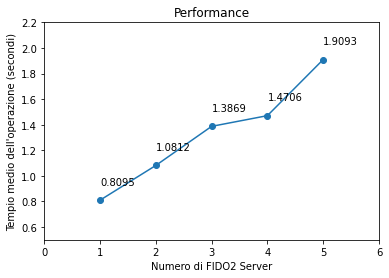
\includegraphics[scale=0.65]{figures/test_results}
\end{center}

Come si può notare dal grafico all'aumentare del numero di FIDO Server l'operazione totale subisce un incremento di circa 20 \emph{ms}. 

I tempi per la fase di registrazione riportano un risultato simile: un incremento di circa 13 \emph{ms} ogni tre FIDO Server aggiuntivi.
\begin{center}
	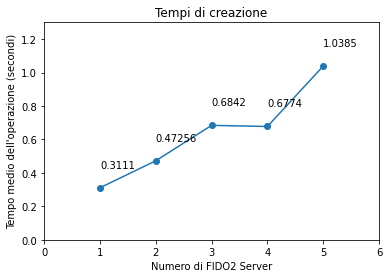
\includegraphics[scale=0.65]{figures/creation_results}
\end{center}

Nella figura successiva sono rappresentati i tempi misurati per la sola fase di autenticazione. Per ogni valore di \emph{k} sono stati utilizzati i valori di security level nel range $[2k+1, 3k+1]$. Come si può notare la variazione del livello di sicurezza, dato lo stesso numero di server malevoli tollerabili, non influenza sensibilmente i tempi dell'operazione.
\begin{center}
	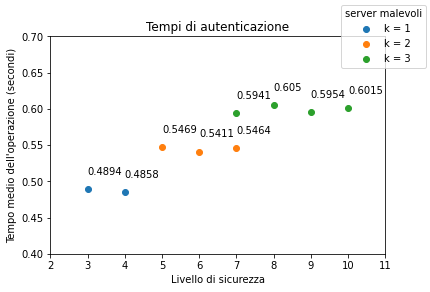
\includegraphics[scale=0.65]{figures/auth_results}
\end{center}

Occorre precisare che le misurazioni effettuate sono assolutamente ottimistiche sia per quanto riguarda la latenza con i FIDO Server, operanti localmente, che per quella con l'autenticatore, emulato virtualmente. Inoltre, non tengono conto dell'interazione umana richiesta e dell'utilizzo di un Web Browser con le penalizzazioni che ne conseguono. 

Si può quindi concludere dai dati raccolti che l'incremento di tempo richiesto dall'operazione con una combinazione di $|Q|$ e \emph{n} è di pochi \emph{ms} in più a fronte di una \emph{survivability} migliore. La parte più onerosa in termini di tempo è quella legata alla registrazione, la quale richiede il doppio del tempo al raddoppiare dei FIDO Server con cui dialogare. La fase di autenticazione, invece, si distanzia di soli $12 ms$ tra il caso limite inferiore e quello superiore considerato, un incremento di circa il $25\%$.

\section{Fattibilità}
\label{fattibilità}

Come specificato nella sezione relativa ai dettagli implementativi \ref{testing}, è stato utilizzato un emulatore dell'autenticatore hardware sviluppato da Solokeys sia per l'implementazione che per la fase di testing. Il codice dell'autenticatore originale è basato sul microcontrollore STM32L432, microcontrollore STM32L432 che offre 256KB di memoria secondaria. L'implementazione suddivide la memoria secondaria nel seguente modo:
\begin{itemize}
	\item 14 KB per il bootloader
	\item 226 KB per il codice da eseguire
	\item 16 KB disponibili per immagazzinare i dati, di cui solo 2048 B adibite alla memorizzazione del contatore
\end{itemize}

Poiché la memoria disponibile è così ridotta gli sviluppatori hanno previsto il cosidetto \emph{wrapping delle chiavi}: invece che generare una coppia di chiavi crittografiche ad ogni richiesta di registrazione, viene generata una singola chiave crittografica \textbf{M} detta \emph{master key} e ad ogni richiesta di registrazione viene computato l'hash di \emph{HMAC(R, M)} dove \textbf{R} è un numero generato al momento. Il risultato dell'hash è una chiave crittografica, da cui verrà derivata la corrispondente chiave pubblica. La prima viene usata per firmare e la seconda viene inviata al server insieme ad \textbf{R}. Nessuna informazione viene salvata dall'autenticatore: l'unico dato necessario all'autenticatore in fase di autenticazione è \textbf{R}, tramite il quale ripeterà il procedimento computando l'\emph{hash} per generare le chiavi. 

Dato che l'implementazione proposta si avvale di una struttura dati \verb*|signCounter| che presenta:
\begin{itemize}
	\item Una struttura dati CredentialID di dimensioni pari a $88$ bytes
	\item Un array di contatori interi senza segno di 16 bit l'uno, i quali garantiscono 1 autenticazione al giorno per 179 anni ($(2^{16}) \div 365$), per 3 livelli di sicurezza
\end{itemize}


Avremo quindi una occupazione di memoria del \verb*|signCounter| di circa $94$ bytes. Per rispettare i vincoli di memoria dell'autenticatore, nella soluzione proposta, come nel firmware dell'autenticatore originale, dedichiamo 2048 bytes alla memorizzazione dei contatori. In questo modo è possibile immagazzinare circa \textbf{21} credenziali differenti. Il risultato ottenuto è in linea con i limiti stabiliti \cite{yubico:resident} da Yubico per le proprie \emph{resident keys}, una tipologia particolare di credenziali che necessitano di essere salvate in memoria.

Occorre considerare che l'aggiunta di un contatore limita le possibilità dell'hardware di fatto riducendo il rapporto costo microcontrollore/numero di credenziali. Si può stimare un costo a contatore ($21$ credenziali * $ 3$ livelli di sicurezza), con un prezzo dell'STM32L432 per grossi stock di $\$4.59673$, di circa $0,07$ cents, sicuramente non trascurabile per grandi numeri.

Viene meno la potenzialità di utilizzare la chiavetta per autenticarsi a virtualmente un numero illimitato di servizi Web ma ciò è compensato dai livelli di sicurezza del tutto sufficienti a garantire un incremento di sicurezza notevole (si parla di una resistenza fino a due server compromessi) e un utilizzo giornaliero costante e duraturo. Considerando anche la limitatezza di servizi Web che offrono l'autenticazione passwordless si può concludere che il limite di ventuno credenziali non è affatto stringente. 
\chapter{Conlusioni}
\label{conclusioni}

Con questa tesi ci si è posto l'obbiettivo di apportare al codice dell'autenticatore Solo e alla libreria FIDO sviluppata da Yubico le opportune modifiche per garantire la \emph{survivability}. La tesi segue la direzione di lavori preesistenti in ambito di autenticazione survivable \cite{magnanini:survivable} e del lavoro già svolto in un'altra tesi precedente sulla libreria FIDO. Proprio in quest'ultima tesi si descrivono risultati conformi a quanto ottenuto in questa sede, ovvero prestazioni adatte a scenari reali di autenticazione distribuita. Ciò è segno che l'aggiunta del livello di sicurezza non costituisce elemento di riduzione delle performance.

La soluzione è stata provata solamente in configurazione locale, motivo per il quale sarebbero necessarie ulteriori analisi prevedendo un autenticatore hardware reale e l'utilizzo di un Browser tramite cui simulare l'interazione dell'utente con un servizio Web. Inoltre, sarebbe interessante studiare la fattibilità per altre tipologie di microcontrollori e il rapporto costi/benefici che deriverebbe dall'adozione rispetto a quello preso in esame. 

% PAGINA VUOTA
%\clearpage\null\thispagestyle{empty}\clearpage
%\appendix
%\appendixpage
%\addappheadtotoc

%\clearpage\null\thispagestyle{empty}\clearpage


%\listoffigures


\begin{flushleft}
\bibliographystyle{plain}
\bibliography{sections/references} 
\end{flushleft}

\end{document}
